\chapter{Daljnji rad}

U prethodnim poglavljima predstavljeni su i implementirani pojedini algoritmi dubokog podržanog učenja koristeći programski jezik \textit{Python}, te primarno biblioteku \textit{PyTorch} za oblikovanje i učenje dubokih modela, te okoline biblioteke \textit{OpenAI Gym} u kojima je agent bio smješten i s kojima je interaktirao i dobivao povratne informacije. Osim obrađenih algoritama dubokog Q učenja, dvostrukog dubokog Q učenja, akter-kritičara, te prednosnog akter-kritičara, u daljnjem radu bilo bi korisno predstaviti, implementirati i isprobati algoritme poput suparničkog dvostrukog Q učenja \engl{Dueling Double Deep Q Network} (skraćeno \textit{D3QN}), asinkronog prednosnog akter-kritičara \engl{Asynchronous Advantage Actor-Critic} (skraćeno \textit{A3C}), mekog akter-kritičara \engl{Soft Actor-Critic} (skraćeno \textit{SAC}), Trust Region Policy Optimization (skraćeno \textit{TRPO}), Proximal Policy Optimization (skraćeno \textit{PPO})... koji u određenim slučajevima daju bolje rezultate od obrađenih algoritama.

Pronalazak optimalnih hiperparametara dubokih modela ovisnima o okolini u kojoj se nalaze je veoma iscrpan i vremenski zahtjevan postupak, no ispravan odabir hiperparametara kao i arhitekture dubokog modela, može uvelike poboljšati performanse agenta. Osim hiperparametara, performanse dubokog modela može poboljšati i korištenje različitih optimizacijskih postupaka. Prilikom implementacije koristio se optimizacijski postupak Adam \engl{Adaptive Moments}, no moguće je koristiti i obični stohastički gradijentni spust \engl{Stohastic Gradient Descent} (skraćeno \textit{SGD}), RMSProp, AdaGrad... i s njima kombinirati upotrebu momenta i restarta kod promjene stope učenja. 

Također, u daljnjem radu korisno bi bilo smjestiti agente te provjeriti kako se ponašaju u novim okolinama i suočavaju s njihovom problematikom. Posebno se zanimljivima čine \textit{OpenAI Gym} okoline \textit{Double Dunk} \cite{DoubleDunk}, \textit{Space Invaders} \cite{SpaceInvaders}, \textit{Car Racing} \cite{CarRacing}, \textit{Pong} \cite{Pong}, te cijela porodica \textit{MuJoCo} okolina za simulaciju i kontrolu. \textit{OpenAI Gym} ima podršku za jednostavan razvoj i ručnu implementaciju novih igara i njihovih okolina, poput igrica \textit{Flappy Bird} \cite{CustomFlappyBird} ili \textit{Dino Game} \cite{CustomDinoGame}.

Podržano učenje ima veliku primjenu i u trgovanju dionicama, valutama \engl{forex}, kriptovalutama za čije bi se treniranje agenata i interakciju mogle koristiti biblioteke \textit{Gym AnyTrading} (slika \ref{fig:gym-anytrading}) \cite{GymAnytrading} i \textit{TensorTrade} \cite{Tensortrade}.

\begin{figure}[H]
    \centering
    \frame{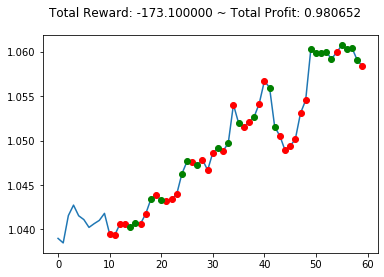
\includegraphics[width=8cm]{assets/gym-anytrading.png}}
    \caption{\textit{Gym AnyTrading} okolina s označenim kupovnim i prodajnim pozicijama}
    \label{fig:gym-anytrading}
\end{figure}
